\documentclass[10pt,letterpaper]{article}
\usepackage{amsmath,amssymb,geometry,graphicx}
\usepackage{enumitem}
%\settextfont{B Nazanin}
\usepackage{lipsum}
\setlength{\parskip}{3mm}
\setlength{\parindent}{0mm}
\newcommand{\wid}{0.49\textwidth}
\newcommand{\widone}{60mm}
\begin{document}
\Large
\begin{center}
In the name of beauty

9th problem set of ComNet course

\hrulefill
\end{center}
Q1)
\begin{enumerate}[label=\alph*-]
\item
False. FEC is also capable of error correction as well as error detection.
\item
False. TDMA and FDMA can be categorized as channel partitioning protocols since the transmission media is split to pre-defined slots, whether in time or frequency. No random access is allowed in these types of protocols.
\item
True. Slotted ALOHA, as the name suggests, requires time slots ALOHA does not. The benefit is doubling the average transmission rate at each node at the cost of more complicated implementation.
\item
False. Link layer switches come with no MAC address. Even if they did, the user has no knowledge about it and to this reason, any of its forwarded frames in the first step will contain a broadcast MAC address in the destination MAC address field.
\end{enumerate}

Q2) The user wishes to be assigned an IP address. It starts by sending a DHCP discover message with src IP address=0.0.0.0, dest IP address=255.255.255.255 on port number 68 to the local switch, src MAC address = self MAC address and dest MAC address = FF:FF:FF:FF:FF:FF. The switch, having no information about the hosts in the LAN (assuming no ARP has been established), learns that the user is available through the interface it received packets from. The switch then, enters suitable information for this userand forwards the frame to all of the other interfaces and users. Since only DHCP is responsible for IP address allocation, all other nodes will finally discard the packet in layer 4 and a 4-step IP address assignment takes place. Finally, the user will be assigned an IP address.

The user is not aware of the MAC address of the first-hop router, hence it includes a broadcast MAC address with the IP address of the corresponding interface of the first-hop router.

Q3) 
The probability that a user sends a packet successfully, is $Np(1-p)^{N-1}$ in slotted ALOHA where $N$ is the number of users and $p$ is the probability of transmission for each user. By defining $q\triangleq Np(1-p)^{N-1}$, the probability that a user sends a packet unsuccessfully $k-1$ times and successfully at its $k$-th transmission is 
$$(1-q)^{k-1}q$$
hence the expected value of the number of transmission becomes 
\begin{equation}
\begin{split}
E&=\sum_{k=1}^{\infty}k(1-q)^{k-1}q
=q\sum_{k=1}^{\infty}k(1-q)^{k-1}
\\&=q{d\over dq}\sum_{k=1}^{\infty}-(1-q)^{k}
=q{d\over dq} -{1-q\over q}
\\&=q{1\over q^2}={1\over q}
={1\over Np(1-p)^{N-1}}
\end{split}
\end{equation}
Q4)
%\begin{center}
%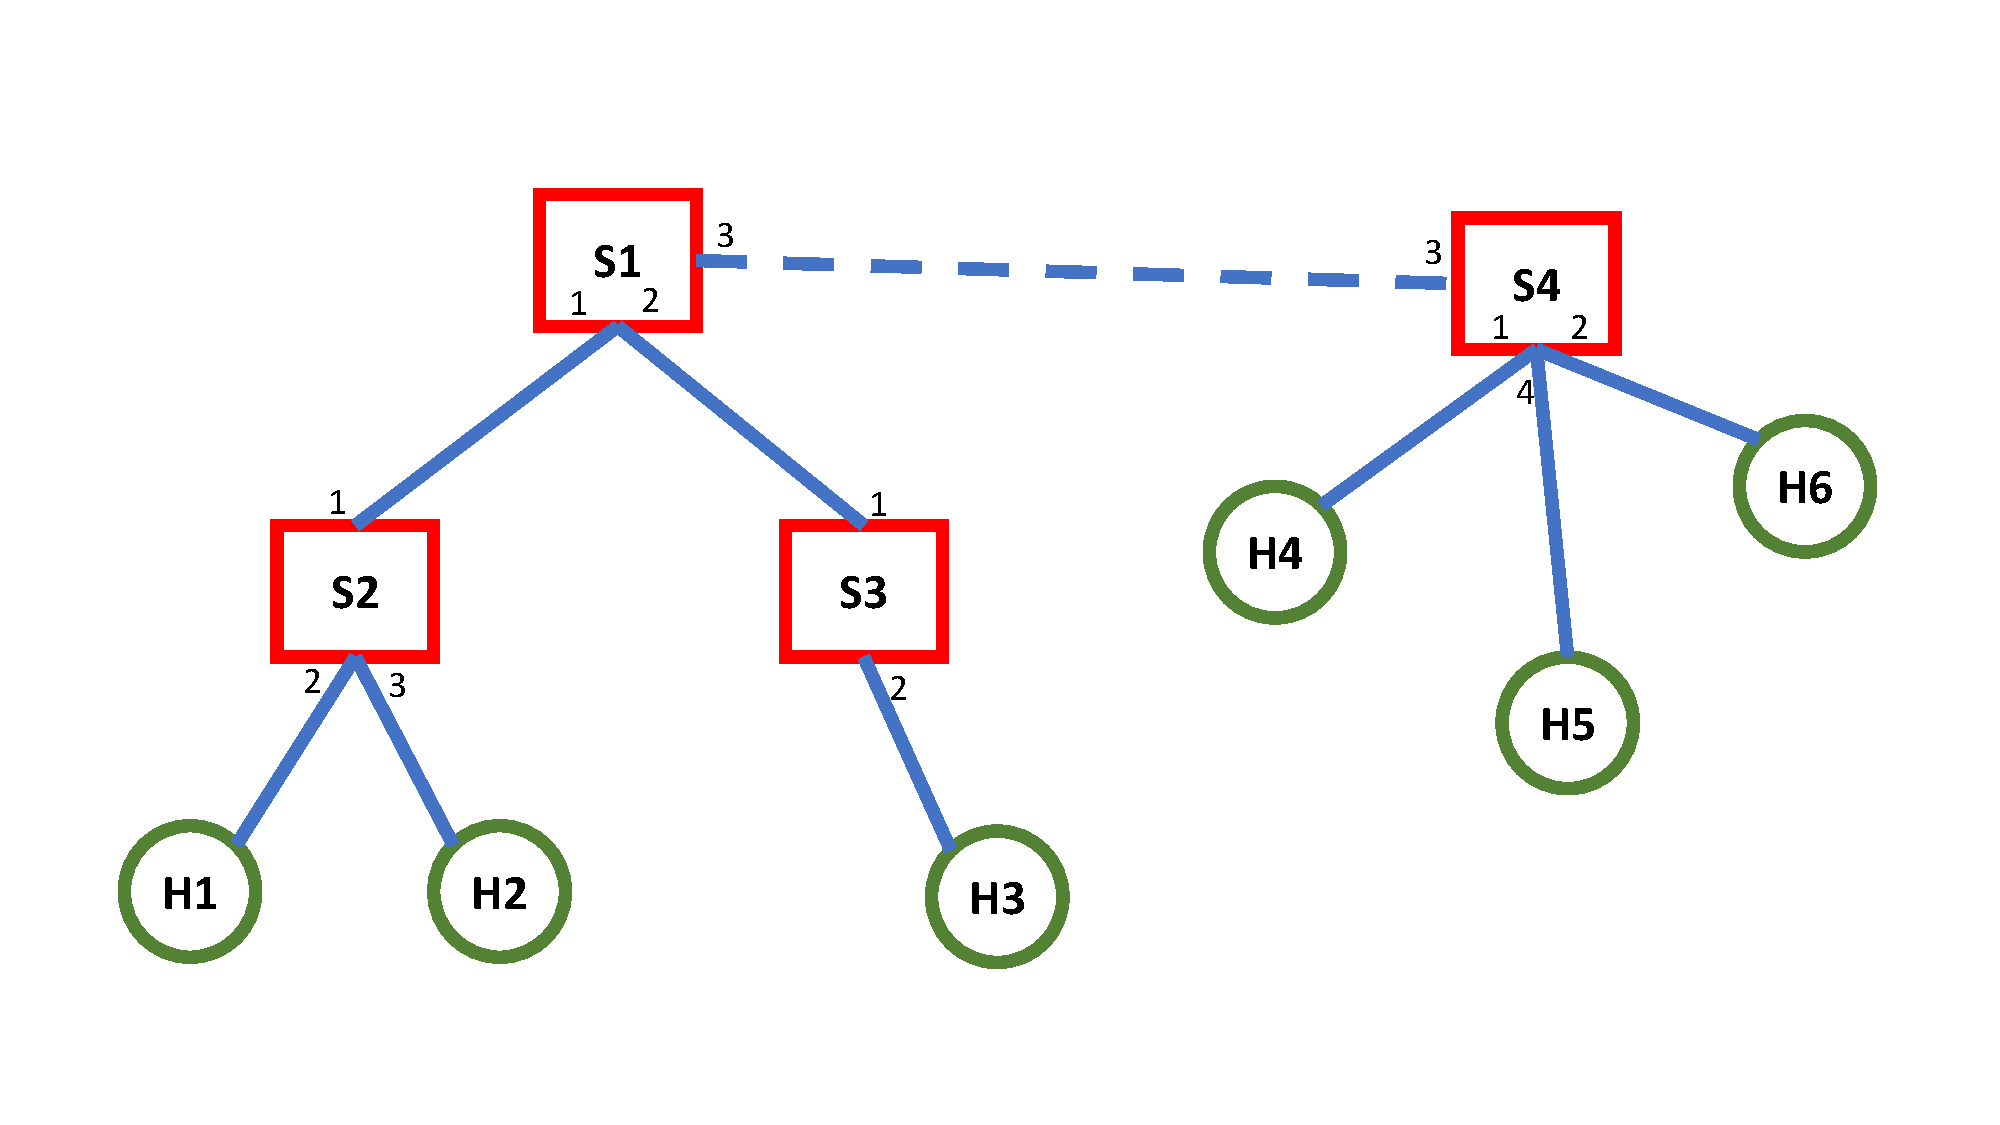
\includegraphics[width=120mm]{Q5_HW8}
%\end{center}
a.

Switch 1 finds out that the MAC address AA:AA:AA:AA:AA:AA is available on port \#1.

Switch 2 finds out that the MAC address AA:AA:AA:AA:AA:AA is available on port \#2.

Switch 3 finds out that the MAC address AA:AA:AA:AA:AA:AA is available on port \#1.

Switch 4 finds out that the MAC address AA:AA:AA:AA:AA:AA is available on port \#3.

b. Since it does not know over which port is H6 available, it forwards the upstream packet to all of its outgoing interfaces.

Q5) Once the packet is in EE department, its destination IP address is that in the CS department and its destination MAC address is set to that of the first-hop router. The source IP and MAC addresses are set to the EE host. The router observes that the frame is headed for it, pulls out the datagram and observes that the destination exists in the CS department. Hence, changes the source MAC address to that of itself, preserves the source IP address (for further addressing or responsing from destination to source), changes the destination MAC address of the frame to that of the destination and preserves the destination IP address.
\end{document}